\documentclass[a4paper,10pt]{article}
\usepackage[utf8]{inputenc}
\usepackage{amsmath,amssymb,graphicx}
\usepackage{tikz}
\usepackage{tikz-3dplot}
\usepackage{xcolor}
\usepackage{hyperref}
\usepackage{geometry}
\geometry{margin=2cm}

\title{\textbf{Simulación: Disparo desde Plataforma Giratoria}}
\author{Física Computacional}

\begin{document}
\maketitle

\begin{abstract}
Este proyecto simula el movimiento de un proyectil disparado desde una plataforma giratoria, comparando las trayectorias en sistemas de referencia inercial y no inercial. Se implementa en C++ con visualización mediante Gnuplot, demostrando los efectos de las fuerzas ficticias (Coriolis y centrífuga) en el sistema rotante.
\end{abstract}

\section{Introducción}
Cuando un proyectil se dispara desde una plataforma en rotación, su trayectoria depende críticamente del sistema de referencia elegido. En el sistema inercial (fijo), el movimiento sigue una parábola simple. En el sistema no inercial (giratorio), aparecen fuerzas ficticias que modifican sustancialmente la trayectoria observada.

\section{Marco Teórico}

\subsection{Sistema Inercial}
En el sistema fijo externo, las ecuaciones de movimiento son:
\begin{align*}
x(t) &= d + v_0\cos\theta\cos\phi \cdot t \\
y(t) &= \omega d \cdot t + v_0\cos\theta\sin\phi \cdot t \\
z(t) &= v_0\sin\theta \cdot t - \frac{1}{2}gt^2
\end{align*}
donde la velocidad inicial incluye la componente tangencial de la rotación.

\subsection{Sistema No Inercial}
En el sistema rotante, las aceleraciones incluyen fuerzas ficticias:
\begin{align*}
a_x &= 2\omega v_y + \omega^2 x \quad \text{(Coriolis + centrífuga)} \\
a_y &= -2\omega v_x + \omega^2 y \\
a_z &= -g \quad \text{(Gravedad)}
\end{align*}

\subsection{Algoritmo Numérico}
\begin{itemize}
\item \textbf{Método}: Integración Euler explícito
\item \textbf{Paso temporal}: $\Delta t$ configurable por usuario
\item \textbf{Condición de parada}: $z \leq 0$ (impacto con el suelo)
\item \textbf{Parámetros}: $\omega, d, v_0, \theta, \phi$ interactivos
\end{itemize}

\begin{figure}[h]
\centering
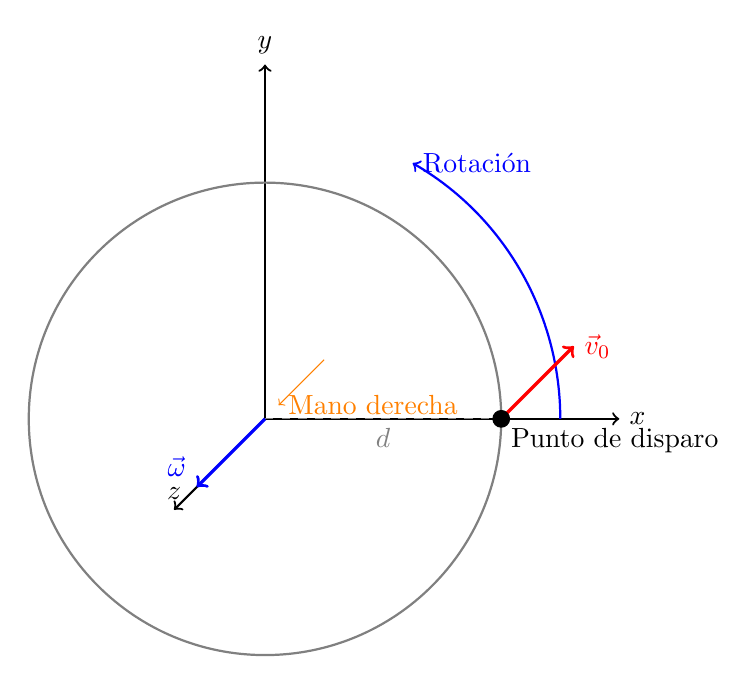
\begin{tikzpicture}[scale=1.5]
% Sistema de coordenadas
\draw[->, thick] (0,0,0) -- (3,0,0) node[right] {$x$};
\draw[->, thick] (0,0,0) -- (0,3,0) node[above] {$y$};
\draw[->, thick] (0,0,0) -- (0,0,2) node[above] {$z$};

% Plataforma circular
\draw[gray, thick] (0,0) circle (2cm);
\draw[gray, dashed] (0,0) -- (2,0) node[midway, below] {$d$};

% Vector velocidad angular
\draw[blue, ->, very thick] (0,0,0) -- (0,0,1.5) node[above left] {$\vec{\omega}$};

% Rotación (indicar dirección)
\draw[blue, ->, thick] (2.5,0) arc (0:60:2.5) node[right] {Rotación};

% Vector velocidad
\draw[red, ->, very thick] (2,0,0) -- (3,1,1) node[right] {$\vec{v}_0$};

% Punto de disparo
\filldraw[black] (2,0,0) circle (2pt) node[below right] {Punto de disparo};

% Regla de la mano derecha
\draw[orange, ->] (0.5,0.5,0) -- (0.5,0.5,1) node[right] {Mano derecha};
\end{tikzpicture}
\caption{Sistema de coordenadas: Plataforma giratoria en el plano $xy$ con velocidad angular $\vec{\omega}$ apuntando en $+z$ (regla de la mano derecha).}
\end{figure}

\section{Convención de Rotación}


\subsection{Implicaciones Físicas}
\begin{itemize}
\item Fuerza de Coriolis: $\vec{F}_C = -2m\vec{\omega}\times\vec{v}$
\item Fuerza centrífuga: $\vec{F}_{cf} = m\omega^2\vec{r}$
\item La dirección de $\omega$ determina el sentido de las desviaciones
\end{itemize}


\section{Resultados y Visualización}

El programa genera:
\begin{itemize}
\item \textbf{Archivos de datos}: Trajectorias completas en ambos sistemas
\item \textbf{Gráficas comparativas}: Posiciones $x(t), y(t), z(t)$ y trayectoria 3D
\item \textbf{Animación}: Visualización 3D con plataforma giratoria
\end{itemize}

\section{Análisis Físico}

\subsection{Efectos Observables}
\begin{itemize}
\item \textbf{Desviación lateral}: Debida a la fuerza de Coriolis
\item \textbf{Alcance diferente}: Entre sistemas inercial y no inercial
\item \textbf{Trayectoria curvada}: En el sistema rotante
\end{itemize}


\section{Conclusión}

Esta simulación demuestra cualitativa y cuantitativamente cómo las fuerzas ficticias modifican la trayectoria de un proyectil en sistemas de referencia no inerciales. El código proporciona una herramienta educativa para visualizar estos efectos fundamentales de la mecánica clásica.

\begin{thebibliography}{9}

\bibitem{price2022}
J.~F. Price, ``A very simple projectile problem analysed from inertial and rotating reference frames'', 
\textit{A Coriolis Tutorial, Part 1}, 2022. Available at: \url{https://www2.whoi.edu/staff/jprice/wp-content/uploads/sites/199/2022/03/aCt-P1-V9.pdf}.

\bibitem{mit2016}
Massachusetts Institute of Technology,
\textit{Chapter 31: Non-Inertial Linear and Rotating Reference Frames},
Course: Classical Mechanics (8.01SC), Fall 2016. Available at: \url{https://ocw.mit.edu/courses/8-01sc-classical-mechanics-fall-2016/mit8_01scs22_chapter31.pdf}.

\end{thebibliography}


\end{document}